\chapter{Extensible Dependency Grammar}\label{XDG}

Extensible Dependency Grammar (XDG) \cite{DebusmannEtal04SS},
\cite{Debusmann06} ist ein Meta-Grammatikformalismus, der auf
Dependenzgrammatik \cite{Tesniere59} basiert, und diese mit
modelltheoretischer Syntax und der parallelen Gram\-matik-Architektur
von Jackendoff \cite{Jackendoff02} kombiniert.

Durch das modulare Design von XDG k\"onnen Grammatiken um jeden
beliebigen linguistischen Aspekt erweitert werden. Die Aspekte, wie
z.B.\ grammatische Funktionen, Wortstellung oder
Pr\"adikat-Argument-Struktur, werden jeweils auf einer eigenen
Dimension behandelt. Die Aufteilung der Aspekte in Dimensionen
erleichtert die Modellierung von linguistischen Ph\"anomenen, da jeder
Aspekt einzeln behandelt wird, und nicht alle Aspekte gleichzeitig
modelliert werden m\"ussen.  Vor allem bei Aspekten, die nicht
voneinander abh\"angen, erleichtert das modulare Design das Entwickeln
von Grammatiken. Zum Beispiel spielt f\"ur die Modellierung der
Pr\"adikat-Argument-Struktur die Wortstellung keine Rolle, im
Gegensatz zu den grammatischen Funktionen. In fr\"uheren Ans\"atzen
musste die Wortstellung jedoch trotzdem bei der Modellierung der
Syntax-Semantik-Schnittstelle miteinbezogen werden.

XDG wird durch eine Multigraph-Beschreibungssprache in
Pr{\"a}dikatenlogik erster Stufe (First-Order Logik)
formalisiert. Eine XDG-Grammatik besteht dabei aus einem
Multigraphtyp, einer Menge von Prinzipien, die die
Wohlgeformtheitsbedingungen des Multigraphen beschreiben, und einem
Lexikon. Nachdem der Multigraphtyp festgelegt ist, werden die
Prinzipien in Abh\"angigkeit des Multigraphtyps in First-Order Logik
beschrieben. Das Lexikon dr\"uckt Eigenschaften von W\"ortern aus.

\section{Multigraphen}

Ein Modell in XDG besteht aus einer Menge von Dependenzgraphen, die
alle die gleiche Menge von Knoten teilen. Dadurch k\"onnen die
Dependenzgraphen zusammen als ein Multigraph aufgefasst werden. Ein
Modell in XDG ist also ein Dependenz-Multigraph.

\subsection{Dependenzgraphen}

\begin{figure}
\centering
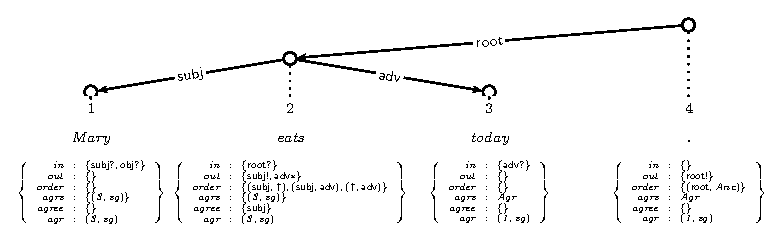
\includegraphics[scale=1.0]{eps/syn1_xdag.eps}
\caption{Dependenzgraph}
\label{DG}
\end{figure}

XDG-Modelle enthalten eine spezielle Form von Dependenzgraphen. Die
Knoten sind hierbei mit einem numerischen Index, beginnend bei 1,
versehen. Dieser Index gibt ihre Position im Eingabesatz
wieder. Au{\ss}erdem wird jeder Knoten mit genau einem Wort des zu
analysierenden Satzes assoziiert, das in Abbildung~\ref{DG} unter dem
Index zu finden ist.  Desweiteren wird jeder Knoten mit Attributen
assoziiert, die in Abbildung~\ref{DG} unter dem Wort stehen. Attribute
modellieren lexikalische und nichtlexikalische Informationen. Die
Knoten werden untereinander durch gerichtete und gelabelte Kanten
verbunden. Die Kantenbeschriftungen dr\"ucken die Beziehungen der
Knoten innerhalb der Dimension aus, z.B.\ syntaktische Funktionen oder
semantische Rollen.

Dependenzgraphen in XDG unterliegen ansonsten keinerlei
Restriktionen. Es wird also nicht verlangt, dass sie Baumform haben
oder \"Ahnliches. Die Dependenzgraphen k\"onnen beliebige Graphen
sein, also auch Graphen mit Zyklen oder kreuzenden Kanten. Das ist
\"ahnlich wie bei Word Grammar (WG) \cite{Hudson90}.

\subsection{Dependenz-Multigraphen}

\begin{figure}
Gegeben:
\begin{itemize}
\item endliche Menge $\mathit{At}$ von Atomen
\item endliche Menge $D$ von Dimensionen
\item endliche Menge $W$ von W\"ortern
\item endliche Menge $L$ von Kantenlabels
\item endliche Menge $A$ von Attributen
\item endliche Menge $T$ von Typen
\end{itemize}
wobei gilt: $D, W, L, A \subseteq \mathit{At}$ und $U = \cup
             \{t|t \in T\}$.

Ein Multigraph ist ein Tupel $(V, E^+, <, \mathit{nw}, \mathit{na})$ bestehend aus:
             \begin{enumerate}
               \item einem endlichen Intervall $V$ aus $\mathbb{N}$ beginnend bei 1, das die
               Knoten rep\"asentiert.
               \item einer endlichen Menge $E^+ \subseteq V \times V \times L \times D$ von gelabelten Dominanzen.
               \item einer strengen Totalordnung $< \subseteq V \times V$
               \item einem Knoten-Wort-Mapping $\mathit{nw} \in V \rightarrow W$

               \item einem Knoten-Attribut-Mapping $\mathit{na} \in V \rightarrow D \rightarrow
               A \rightarrow U$.
             \end{enumerate}
             
\caption{Multigraph formal}
\label{multiformal}
\end{figure}

Die verschiedenen Dependenzgraphen eines Modells k\"onnen als
Multigraph aufgefasst werden, da sie dieselbe Knotenmenge
teilen. Jeder Dependenzgraph beschreibt eine andere Dimension.

Formal ist ein Multigraph in XDG definiert wie in
Abbildung~\ref{multiformal}. Die Dimensionen $D$, die W\"orter $W$, die
Kantenlabel $L$ und die Attribute $A$ sind endliche Mengen von Atomen $\mathit{At}$.
Desweiteren gibt es eine endliche Menge von Typen $T$ und eine Menge von
Werten $U$. Werte sind immer Mengen von Tupeln \"uber endlichen Mengen
von Atomen.

$V$ sind die Knoten des Multigraphen, duchnummeriert beginnend mit
1. Der Index gibt die Position des Knotens im Satz an.

Die Menge $E^+$ beschreibt indirekt die Kanten des Graphen, wobei
gilt, dass $(v, v', l, d) \in E^+ $ gdw. der Graph in der Dimension $d$
eine Kante von $v$ nach $v''$ hat, die mit $l$ gelabelt ist, und dann 0
oder mehr Kanten von $v''$ nach $v'$. Die Elemente von $E^+$
hei{\ss}en \emph{gelabelte Dominanzen}. Gelabelte Dominanzen haben den
Zweck, die transitive H\"ulle der Kantenrelation fix ins Modell zu
kodieren, weil diese nicht innerhalb von First-Order Logik
ausgedr\"uckt werden kann. Eine andere Option w\"are es, in Modellen
nur Kanten zu kodieren, und die transitive H\"ulle \"uber
Erweiterungen der Logik (Fixpunkte, Logik zweiter Stufe) zu
erreichen. Daf\"ur gibt es allerdings bis dato keine weiteren
Gr\"unde.

Das Knoten-Wort-Mapping weist jedem Knoten aus $V$ ein Wort aus $W$ zu.

Das Knoten-Attribut-Mapping weist jedem Knoten f\"ur jede Dimension
die passende Attribute zu.

Der {\it Multigraphtyp} legt die m\"oglichen Dimensionen, W\"orter,
Kantenlabels und Knotenattribute fest. Der Multigraphtyp ist ein Tupel
$\mathit{MT} = (D,W,L,\mathit{dl},A,T,\mathit{dat})$. Die Dimensionen $D$, die W\"orter $W$ und die Labels
$L$ sind endliche Mengen aus Atomen. Das Dimension-Label-Mapping $\mathit{dl} \in
D \rightarrow 2^L$ legt fest, welche Kantenbeschriftungen aus $L$ f\"ur
die Dimensionen m\"oglich sind, und das
Dimensions-Attribut-Typ-Mapping, welche Attribute mit welchen Werten.

Es gilt, ein Multigraph $M = (V, E ^ + , < , \mathit{nw}, \mathit{na} )$ der auf den
Dimensionen $D'$, den W\"ortern $W'$, den Kantenlabels $L'$, den
Attributen $A'$ und den Typen $T'$ definiert ist, hat den
Multigraphtyp $\mathit{MT} = (D,W,L,\mathit{dl},A,T,\mathit{dat})$ gdw. $D'= D$, $W' \subseteq W$,
$L' \subseteq L$, $A' = A$, $T' = T$, alle Kanten in Dimension $d \in
D'$ haben nur Kantenbeschriftungen in $dl d$, und alle Knotenattribute
$a \in A'$ in Dimension $d \in D'$ haben Werte in $\mathit{dat} d a$, d.h. die,
womit sie wohlgetypt sind.

\section{Grammatiken}

\begin{figure}
Grammatik $G = (\mathit{MT}, \mathit{lex}, P)$ mit
\begin{enumerate}
  \item $\mathit{MT}$ := Multigraphtyp
  \item $\mathit{lex}$ := Lexikon
  \item $P$ := Menge von Prinzipien
\end{enumerate}
$P$ und $\mathit{lex}$ sind auf dem gleichen Multigraphtype $\mathit{MT}$ definiert.
\caption{XDG Grammatik formal}
\label{gramformal}
\end{figure}

Mengen von Modellen in XDG werden durch Grammatiken beschrieben.  Eine
Grammatik besteht wie in Abbildung~\ref{gramformal} aus einem
Multigraphtyp $\mathit{MT}$, einem Lexikon $\mathit{lex}$ und einer
Menge von Prinzipien $P$. F\"ur $\mathit{lex}$ und $P$ gilt, dass sie
auf $\mathit{MT}$ definiert sind, also auf dem gleichen Multigraphtyp.

\subsection{Die Beispielgrammatik CSD}
\begin{figure}
\centering
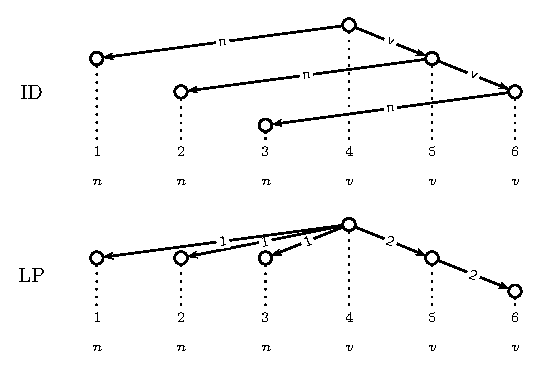
\includegraphics[scale=1.0]{eps/nnnvvv.eps}
\caption{Beispielanalyse der CSD-Grammatik f\"ur die Eingabe ``nnnvvv''}
\label{csdanalyse}
\end{figure}
An dieser Stelle wollen wir eine Grammatik vorstellen, auf die wir im
Laufe dieser Arbeit immer wieder zur\"uckkommen werden.  Die Grammatik
CSD (Cross-Serial-Dependencies) beschreibt die Wortketten:
$$
\text{CSD} = \{n^{1} \ldots n^{k} v^{1} \ldots v^{k} \mid k \geq
1 \}
$$ Also S\"atze mit $k$ Nomen $n$, gefolgt von $k$ Verben $v$. Eine
Analyse f\"ur den Satz {\it nnnvvv} zeigt Abbildung~\ref{csdanalyse}. Jedes Nomen und
jedes Verb ist mit einem Index $i$ mit $1 \leq i \leq k$ versehen, und
es muss gelten, dass das Nomen $n^{i}$ ein Argument des Verbes $v^{i}$
ist. Solche Satzkonstruktionen k\"onnen nicht mehr mit kontextfreien
Grammatiken modelliert werden und kommen z.B.\ in Nebens\"atzen des
Holl\"andischen vor, z.B.:
\begin{center}
{\it
\begin{tabular}{c c c c c c c c c}
(omdat) & ik & Cecilia & Henk & de & nijlpaarden & zag & helpen &
voeren \\
(dass) & ich & Cecilia & Henk & die & Nilpferde & sah & helfen &
f\"uttern \\
\multicolumn{8}{c}{{\it``(dass) ich Cecilia Henk die Nilpferde f\"uttern sah''}}
\end{tabular}
}
 \end{center}

Der Multigraphtyp $\mathit{MTCSD} = (D,W,L,\mathit{dl},A,T,\mathit{dat})$ der Grammatik hat die
Dimensionen {\tt ID} und {\tt LP}, die W\"orter {\tt n} und {\tt v}
sowie die Menge $L=\{\mathtt{n},\mathtt{v},\mathtt{1},\mathtt{2}\}$.  {\tt ID} steht dabei f\"ur
\emph{Immediate Dominance} und {\tt LP} f\"ur \emph{Linear
Precedence}, in Analogie zu GPSG \cite{GazdarEtal85}.  Das Mapping
$\mathit{dl}$ legt fest, dass {\tt n} und {\tt v} f\"ur die Dimension {\tt
ID} verwendet werden, {\tt 1} und {\tt 2} f\"ur die Dimension {\tt
LP}. Die Menge der Attribute $A$ ist ${\mathtt{in},\mathtt{out},\mathtt{order}}$ wobei {\tt in} und
{\tt out} den Typ $2^{L\times\{!,?,*,+\}}$ haben, womit beschrieben
wird, wieviele eingehende/ausgehende Kanten mit einem bestimmten Label
erlaubt sind.  {\tt order} hat den Typ $2^{L\times L}$, womit eine
Ordnung auf den Kantenlabels beschrieben wird.

\subsection{Lexikon}
 
%% \begin{figure}
%% $$
%% \text{wants} \mapsto
%% \left \{
%% \left \{
%% \begin{array}{r c l}
%% SYN & : & \left \{ 
%% \begin{array}{r c l}
%% in & : &\{root?\}\\
%% out & : & \{subj!, vinf!, adv* \} \\
%% \end{array}
%% \right \} \\
%% SEM & : & \left \{ 
%% \begin{array}{r c l}
%% in & : &\{root!, th*\}\\
%% out & : & \{ag!, th! \} \\
%% \end{array}
%% \right \} \\
%% \end{array}
%% \right \} \quad , \quad \ldots \quad \right \}
%% $$
%% \caption{Beispielhafter Lexikoneintrag f\"ur das Wort 'wants'}
%% \label{lexiconexample}
%% \end{figure}

\begin{figure}
\centering
\begin{tabular}{c c c c c}
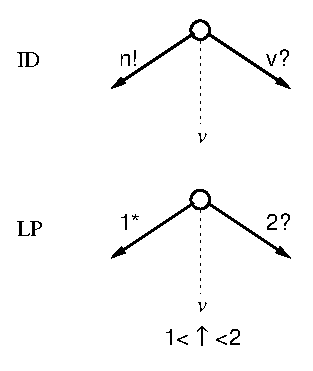
\includegraphics[scale=0.7]{eps/csd_v1_fig}& 
\vspace{1cm} &
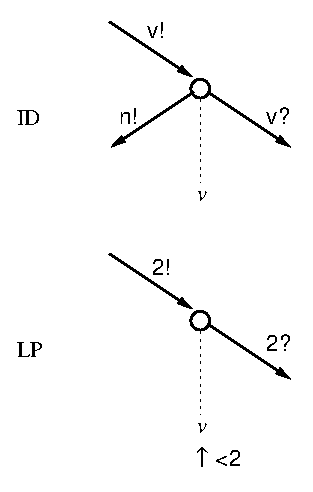
\includegraphics[scale=0.7]{eps/csd_v2_fig}& 
\vspace{1cm} &
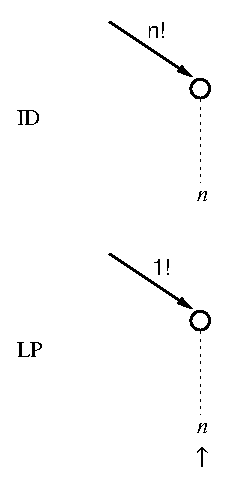
\includegraphics[scale=0.7]{eps/csd_n_fig}   \\
(a) & & (b) & & (c)
\end{tabular}
\caption{Schematische Darstellung des Lexikons der CSD-Grammatik}
\label{csdlexicon}
\end{figure} 

   
\begin{figure}
$$
\text{v} \mapsto
\left \{
\begin{array}{c}
\left \{
\begin{array}{r c l}
ID & : & \left \{ 
\begin{array}{r c l}
in & : &\{\}\\
out & : & \{n!, v? \} \\
\end{array}
\right \} \\
LP & : & \left \{ 
\begin{array}{r c l}
in & : &\{\}\\
out & : & \{1*, 2? \} \\
order & : & \{(1, \uparrow , 2)\}
\end{array}
\right \} \\
\end{array}
\right \} , \\
\left \{
\begin{array}{r c l}
ID & : & \left \{ 
\begin{array}{r c l}
in & : &\{v!\}\\
out & : & \{n!, v? \} \\
\end{array}
\right \} \\
LP & : & \left \{ 
\begin{array}{r c l}
in & : &\{2!\}\\
out & : & \{2? \} \\
order & : & \{( \uparrow , 2)\}
\end{array}
\right \} \\
\end{array} 
\right \} , \\
\ldots
\end{array}
 \right \}
$$
\caption{Die Lexikoneintr\"age f\"ur ein Verb der CSD-Grammatik in
konkreter Form}
\label{csdlexiconexample}
\end{figure}

Das Lexikon bildet W\"orter auf Mengen von Lexikoneintr\"agen ab. Ein
Lexikoneintrag legt die Werte der lexikalischen Attribute der
jeweiligen Dimensionen fest. %In Abbildung~\ref{lexiconexample} sieht
%man einen Lexikoneintrag f\"ur das englische Wort 'wants', in dem die
%'in' und 'out' Attribute f\"ur die Dimensionen SYN und SEM
%spezifiziert werden.
%
In Abbildung~\ref{csdlexicon} sieht man die Lexikoneintr\"age f\"ur
die Nomen und Verben der CSD Grammatik in schematischer Darstellung,
und Abbildung~\ref{csdlexiconexample} zeigt die beiden
Lexikoneintr\"age f\"ur das Verb {\tt v} in konkreter Form als
Records. Teil (a) von Abbildung~\ref{csdlexicon} besagt, dass falls
das Verb die Wurzel ist (d.h.\ keine eingehende Kante hat), muss es auf
Dimension {\tt ID} genau eine ausgehende Kante mit Beschriftung {\tt n}, und auf
Dimension {\tt LP} beliebig viele ausgehende Kanten mit Beschriftung
{\tt 1}
haben. Die Dependenten, die durch diese Kanten bezeichnet werden,
m\"ussen links vom Verb (markiert mit $\uparrow$) stehen. Rechts vom
Verb ist auf {\tt ID} und {\tt LP} h\"ochstens ein Dependent, der mit einer Kante
mit Beschriftung {\tt v} bzw.\ {\tt 2} verbunden ist, erlaubt.  Teil (b)
beschreibt Verben, die als Dependent vorkommen. F\"ur diese wird
zus\"atzlich zu den Kanten aus Teil (a) noch genau eine eingehende
Kante von mit Beschriftung {\tt v} bzw.\ {\tt 2} verlangt, sie erlauben jedoch auf
{\tt LP} keine ausgehenden Kanten mit Label {\tt 1}. Die Ordnung $\uparrow < 2$
fordert, dass 2-Dependenten rechts des Knotens vorkommen.  Teil (c)
fordert f\"ur Nomen, dass sie auf beiden Dimensionen Dependent eines
Knotens sein m\"ussen. Die Kante muss mit {\tt n} bzw.\ {\tt 1} beschriftet
sein. Nomen k\"onnen keine ausgehenden Kanten haben.

\subsection{Prinzipien}
\begin{figure}
$$ t ::= c | x$$
$$\phi ::= \neg \phi | \phi_1 \wedge
            \phi_2 | \exists x : \phi | t_1 = t_2 | \psi $$
            $$
            \begin{array}{r c l}
            \psi & ::= & v < v' \\
                & | & v \overset{l}{\rightarrow_d}\rightarrow_d^* v' \\
                & | & w(v) = w \\
                & | & (t_1 \ldots t_n) \in a_d (v)
            \end{array}
            $$
\caption{Terme, Formeln und Pr\"adikate }
\label{termpred}
\end{figure}

\begin{figure}
$$
\begin{array}{r c l c}
tree_d & = & \forall v: \neg (v \rightarrow_d^+ v) \wedge & (1)\\
       &   & \exists ! v: \neg \exists v' : v' \rightarrow_d v
       \wedge & (2)\\
       &   & \forall v : (( \neg \exists v' : v' \rightarrow_d
       v) \vee (\exists ! v' : v' \rightarrow_d v)) \wedge & (3)\\
       &   & \forall v: \forall v': \forall l : \forall l' : v
       \overset{l}{\rightarrow}_d \rightarrow_d^* v' \wedge v
       \overset{l'}{\rightarrow}_d \rightarrow_d^* v' 
       \Rightarrow l = l' & (4)\\
      &   &  & \\
csd_d & = & \forall v, v': & \\
      &   & v \overset{n}{\rightarrow}_d v' \Rightarrow \forall
      v'', v''': v'' \rightarrow^+_d v \wedge v''
      \overset{n}{\rightarrow}_d v''' \Rightarrow v''' < v' &  
\end{array}$$

\caption{Das Tree-Prinzip und das CSD-Prinzip}
\label{treeprinciple}
\end{figure}

Die Prinzipien sind das zentrale Element in XDG. Durch Prinzipien
werden die Wohlgefomtheitsbedingungen der XDG-Modelle ausgedr\"uckt.
Ein Multigraph ist genau dann wohlgeformt, wenn er alle Prinzipien der
Grammatik erf\"ullt.

Ein Grammatikschreiber kann entweder neue Prinzipien selbst schreiben,
oder Prinzipien aus einer vordefinierten Prinzipienmenge ausw\"ahlen,
der \emph{Prinzipienbibliothek}.  Typische Prinzipien hieraus sind
z.B.\ das Tree-Principle, das fordert, dass der Dependenzgraph einer
bestimmten Dimension Baumform hat. Der Dependenzgraph darf also nur
eine Wurzel haben, jeder Knoten hat genau eine Mutter oder keine
Mutter, der Dependenzgraph darf keine Zyklen enthalten, und die
Teilb\"aume unterhalb eines Knotens mit verschiedenen Labels sind
disjunkt. Ein weiteres wichtiges Prinzip ist das Valency-Principle,
das in Abh\"angigkeit des Lexikons die m\"oglichen ein- und
ausgehenden Kanten eines Knotens festlegt.

Formalisiert werden die Prinzipien in First-Order Logik. Dabei gilt,
dass die Prinzipien lexikalisiert sein k\"onnen, also in
Abh\"angigkeit des Lexikons stehen k\"onnen, wie z.B.\ das
Valency-Principle, das die m\"oglichen ein- und ausgehenden Kanten
jedes Wortes in dessen Lexikoneintr\"agen definiert. Das
Valency-Principle stellt sicher, dass die Kanten des Multigraphen nach
den Spezifikationen des Lexikons zul\"assig sind.

Formal ist ein Prinzip $p$ eine First-Order-Formel aus der Formelmenge
$\phi$, die \"uber Termen gebildet wird. $\phi$ ist definiert wie in
Abbildung~\ref{termpred}, wobei die hier fehlenden, \"ublichen
logischen Operatoren bzw.\ Quantoren $\vee$, $\Rightarrow$,
$\Leftrightarrow$, $\forall$, $\exists !$ und $\neq$ mit Hilfe der Formeln
aus $\phi$ hergeleitet werden k\"onnen. Sie werden daher in XDG als
syntaktischer Zucker bereitgestellt.

Ein Term $t$ ist entweder eine Individuenkonstante oder eine
Individuenvariable.  Die Individuenkonstanten sind in Bezug auf den
Multigraphtyp $\mathit{MT} = (D,W,L,\mathit{dl},A,T,\mathit{dat})$ Elemente aus der Menge $C = D
\cup W \cup L \cup A \cup F \cup \mathbb{N}$, also Dimensionen,
W\"orter, Kantenbeschriftungen, Attribute, Komponenten von
Attributwerten und Knoten.  Komponenten von Attributwerten werden
durch die Menge $F = \cup \{\mathit{Fd}_{1} \cup \ldots \cup \mathit{Fd}_n | 2^{\mathit{Fd}_1
\times \ldots \times \mathit{Fd}_n} \in T\}$ dargestellt.  Individuenvariablen
k\"onnen z.B.\ Knotenvariablen, Wortvariablen usw.\ sein.

Um \"uber die Multigraph-Modelle sprechen zu k\"onnen, stellt die
Logik in XDG einige vordefinierte Pr\"adikate $\psi$
(Abbildung~\ref{termpred}) zur Verf\"ugung. Hierbei ist die
Interpretation des Pr\"adikats $<$ die strenge totale Ordnung von $V$
definiert aus dem Multigraph.  Das Pr\"adikat $v
\overset{l}{\rightarrow}_d \rightarrow_d^* v'$ steht f\"ur eine
gelabelte Dominanz, d.h.\ einen Pfad in Dependenzgraphen der Dimension
$d$ vom Knoten $v$ zum Knoten $v'$ mit mindestens einer Kante. Die erste
Kante in diesem Pfad muss die Kantenbeschriftung $l$ haben.  $w(v) = w$
vergleicht eine Individuenkonstante $w$ aus $W$ mit dem Wort, mit dem der
Knoten $v$ \"uber das Node-Word-Mapping assoziiert ist. $(t_1 \ldots
t_n) \in a_d(v)$ pr\"uft, ob das Tupel $(t_1 \ldots t_n)$ ein Element
des Attributs $a$ auf Dimension $d$ des Knotens $v$ ist.

Drei Shortcuts werden vereinbart, um weitere Kantenbeziehungen zu
beschreiben:
$$ v \rightarrow _d ^+ v' \overset{\mathit{def}}{=} \exists l: v
\overset{l}{\rightarrow}_d \rightarrow_d^* v'$$
definiert einen Pfad von $v$ nach $v'$ der L\"ange mindestens eins,
allerdings mit beliebiger Kantenbeschriftung.
$$v \overset{l}{\rightarrow}_d v' \overset{\mathit{def}}{=} v
\overset{l}{\rightarrow}_d \rightarrow_d^* v' \wedge \neg \exists v''
: v \rightarrow_d^+ v'' \wedge v'' \rightarrow_d^+ v'$$ beschreibt
einen Pfad der L\"ange eins mit Kantenbeschriftung $l$ von $v$ nach $v'$
(d.h.\ eine gelabelte Kante) in Dimension $d$, indem verlangt wird, dass
es keinen Knoten $v''$ zwischen $v$ und $v'$ geben darf.

$$v \rightarrow v' \overset{\mathit{def}}{=} \exists l : v
\overset{l}{\rightarrow}_d v'$$ verlangt eine Kante von $v$ nach $v'$
in Dimension $d$ mit beliebiger Kantenbeschriftung.

Damit sind die Prinzipien vollst\"andig spezifiziert. Neue Prinzipien
k\"onnen also in First-Order Logik definiert werden, wie in
Abbildung~\ref{treeprinciple} als Beispiel zu sehen ist. Zu sehen ist
das Baumprinzip, das unter anderem von der CSD Grammatik verwendet
wird. Die erste Zeile beschreibt die Eigenschaft, dass ein Baum keine
Zyklen enthalten darf, indem f\"ur alle Knoten gelten muss, dass es
keinen Pfad zu sich selbst gibt. Die zweite Zeile besagt, dass es
genau einen Knoten gibt, der keinen Vorg\"anger hat, also die Wurzel
ist. Dieser Knoten darf nicht am Ende eines Pfades liegen. Zeile drei
verlangt, dass jeder Knoten h\"ochstens einen Mutterknoten hat.  Die
vierte Zeile stellt sicher, dass zwei Unterb\"aume eines Knotens mit
unterschiedlicher Beschriftung disjunkt sind. Damit stellt man auch
sicher, dass es zwischen zwei Knoten nicht mehr als eine Kante gibt.

Die CSD Grammatik verwendet folgende Prinzipien:
\begin{itemize}
\item auf {\tt ID}: Tree-Prinzip, Valency-Prinzip und CSD-Prinzip
\item auf {\tt LP}: Tree-Prinzip, Valency-Prinzip und Order-Prinzip
\item auf {\tt ID} und {\tt LP}: Climbing-Prinzip.
\end{itemize}
W\"ahrend das Tree-Prinzip und Valency-Prinzip typische Prinzipien
sind, und daher sp\"ater f\"ur die Implementierung einfach aus einer
Prinzipienbibliothek ausgew\"ahlt werden k\"onnen, ist das CSD-Prinzip
ein speziell f\"ur diese Grammatik entwickeltes Prinzip, das
sicherstellt, dass alle {\tt n}-Dependenten eines Verbes $v$ nach den
{\tt n}-Dependenten der Verben \"uber $v$ (die $v$ dominieren) folgen
m\"ussen. In Abbildung~\ref{treeprinciple} ist das CSD-Prinzip als
Formel in First-Order Logik zu sehen.

\subsection{Modelle}

Modelle einer Grammatik $m\ G = (\mathit{MT}, \mathit{lex}, P)$ sind
alle Multigraphen $M$, f\"ur die gilt:
\begin{enumerate}
\item $M$ hat Multigraphtyp $\mathit{MT}$
\item $M$ erf\"ullt das Lexikon $\mathit{lex}$
\item $M$ erf\"ullt alle Prinzipien $P$
\end{enumerate}

Ein Multigraph $M=(V, E^+, <, \mathit{nw}, \mathit{na})$ beschreibt
einen String $s\ M = \mathit{nw}~p_1 \ldots \mathit{nw}~ p_n$, wobei
f\"ur $1 \leq i < j \leq n: (p_i, p_j) \in <$. Die Stringsprache einer
Grammatik ist dann $L\ G=\{s\ M|M \in m\ G\}$.

Ein Eingabestring $S=a_1 \ldots a_n$ ist in $L\ G$, wenn es ein Modell
mit einer Knotenmenge $V=\{1, \ldots , n\}$ gibt, f\"ur die gilt, dass
f\"ur alle $v \in V: \mathit{nw}~v \rightarrow a_v$ und $< = 1 <
\ldots < n$.

\section{Eigenschaften}

\subsection{Ausdrucksst\"arke}

Zur M\"achtigkeit von XDG kann gesagt werden, dass alle kontextfreien
Grammatiken von XDG beschrieben werden k\"onnen \cite{Debusmann06}.
Das ist aber nicht alles. XDG kann noch weitere Sprachen aus dem
Bereich der schwach-kontextsensitiven Sprachen beschreiben, z.B.\ die
Sprache $A^N B^N C^N \ldots $ (mit beliebig vielen Bl\"ocken der
L\"ange $N$).  Die Grammatikformalismen TAG und CCG k\"onnen nur
Sprachen mit vier Bl\"ocken beschreiben. Desweiteren kann XDG sogar
Ph\"anomene modellieren, die von keinem schwach-kontextsensitiven
Grammatikformalismus abgedeckt werden, z.B.\ Scrambling
\cite{Debusmann07MTS}. Ein Beweis, dass XDG regul\"are
Dependenzgrammatiken \cite{KuhlmannMoehl07}, \cite{Kuhlmann07}
modellieren kann und damit auch Linear Context-Free Rewriting Systems
(LCFRS) ist laut Ralph Debusmann zwar noch nicht publiziert, aber
fertig.

\subsection{Abschlusseigenschaften}

Die durch XDG beschreibbaren Sprachen sind abgeschlossen unter
Vereinigung und Schnitt, nicht jedoch unter Komplement
\cite{Debusmann07MTS}.

\subsection{Komplexit\"at}      

Das universelle Erkennungsproblem von XDG ist PSPACE-vollst\"andig,
das fixe Erkennungsproblem NP-vollst\"andig \cite{Debusmann07FG}.
